\begin{center}	
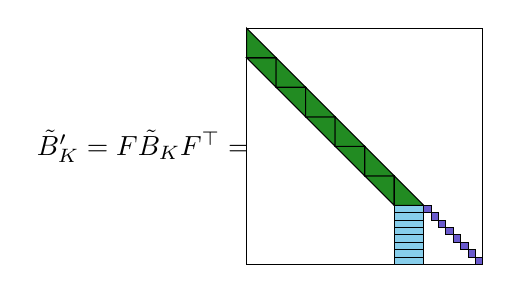
\begin{tikzpicture}[scale=.75]
  \pgfmathsetmacro{\isx}{.125}
  \pgfmathsetmacro{\ix}{.5}
  \begin{scope}
    \draw (0,0) node{$\tilde{B}_K^\prime = F \tilde{B}_K F^\top =$};
  \end{scope}
  \begin{scope}[shift={(0:1.75)}]
    \draw[fill=white] (0,-2) rectangle +(4,4);
    %% diagonal elements
    \foreach \x in { 24,...,31 }
    \draw[fill=SlateBlue] (\x*\isx,2-\isx-\x*\isx) rectangle +(\isx,\isx);
    %% rectangular
    %% \draw[fill=PaleVioletRed] (1,1) rectangle +(\ix,8*\isx);
    \foreach \x in { 0,...,7 }
    \draw[fill=SkyBlue] (2.5,-2+\x*\isx) rectangle +(\ix,\isx);
    %% \draw (1,-1.25) node{$\overline{B}_k$};
    %% block diagonal elements
    \foreach \x in { 0,...,4 }
    \draw[fill=ForestGreen] (\x*\ix+\ix,2-2*\ix-\x*\ix) -- (\x*\ix+\ix,2-2*\ix-\x*\ix+\ix) -- (\x*\ix,2-2*\ix-\x*\ix+\ix) -- cycle;
    %% block sub-diagonal elements
    \foreach \x in { 1,...,6 }
    \draw[fill=ForestGreen] (\x*\ix,2-\x*\ix) -- (\x*\ix-\ix,2-\x*\ix) -- (\x*\ix-\ix,2-\x*\ix+\ix) -- cycle;
  \end{scope}
\end{tikzpicture}
\end{center}

